% ************ Chapter 5 ************
\chapter{Implementação e validação} 
\label{cap:5}
Neste capítulo são apresentadas as fases de desenvolvimento e a validação do projeto. No final é ainda apresentada uma lista das ferramentas utilizadas no projeto.

\section{Desenvolvimento do projeto}
A primeira fase do projeto foi desenvolvida entre as semanas 4 e 6. Este desenvolvimento consistiu criar os modelos (\textit{models}), desenhar cada um dos ecrãs das aplicação (\textit{views}) e os controladores (\textit{controllers}) dos casos de uso Marcar Ponto, Registo de Recolha, Registo de Produção, Registo de Produto Acabado e Registo de Saída de Produto Acabado.\\
Utilizando os recursos do \textit{framework} Laravel, os \textit{models} foram gerados automaticamente com base na estrutura da base de dados, através do recurso de \textit{migrations}. As \textit{migrations} são um ficheiros que descrevem a estrutura de uma tabela da base de dados. Estes servem para poder criar ou alterar tabelas na base de dados sem que o programador tenha de se preocupar com o DBMS.\\
O Laravel inclui o Artisian, uma interface de linha de comandos que disponibiliza uma um conjunto de uteis para a construção da aplicação\cite{Laravelb}.
Para criar uma \textit{migration} e o seu respetivo \textit{model} basta executar no terminal o seguinte comando

\begin{lstlisting}
$ php artisian make:migration NomeDaMigration -m
\end{lstlisting}

\noindent
E serão gerados os ficheiros de \textit{migration} e \textit{model}. Após inserir a estrutura que se pretende para as tabelas da base de dados e suas relações nos ficheiros de \textit{migrations}, usando o comando

\begin{lstlisting}
$ php artisian migrate
\end{lstlisting}

\noindent
As tabelas da base de dados seriam criadas exatamente da forma como foram descritas.\\
Finalizada a criação dos \textit{models}, iniciou-se o processo de desenho de cada uma das \textit{views}. Nesta fase já se sabia que muitos elementos se iriam repetir ao longo da interface, uma consequência direta da coesão da interface. Por esse motivo procurou-se desde cedo isolar alguns elementos de cada um dos ecrãs, como descrito na figura \ref{fig:ui_fabrica_camadas}, para que evitar reescrever código, além de simplificar futuro trabalho de manutenção. Definiu-se então que todas as páginas seriam construídas em cima de uma mesma base. Dependendo da página solicitada era incluída a \textit{view} a ela referente. No caso dos formulários era ainda incluídos os botões de ação (Guardar, Limpar e Cancelar), com a excepção do formulário de Registo de Ponto. Por fim, os elementos de \textit{dropdown} de seleção de Colaborador e Ponto de Recolha eram ainda incluídos de outros dois ficheiros independentes. 
\begin{figure}[htbp] 
	\begin{center}
		% Requires \usepackage{graphicx}
		\includegraphics[width=\textwidth,keepaspectratio]{figuras/camadas_fabrica.png}
		\caption{Camadas da página Aplicação Fábrica}
		\label{fig:ui_fabrica_camadas} 
	\end{center}
\end{figure}

\noindent
Estas inclusões de ficheiros foram produzidas através do recurso Blade do Laravel. O Blade é um mecanismos de modelagem incluso no Laravel que ao contrario da maioria dos mecanismos de modelagem permite o uso de código PHP na própria \textit{view}. São ficheiros com a extensão \textit{.blade.php} e estão, normalmente, dentro do diretório \textit{resources/views}\cite{Laravela}.Para utilizar este recurso do \textit{framework} Laravel é necessário usar um template que tenha sido compatibilizado com este. O template utilizado foi o AdminLTE\cite{AlmsaeedStudio} implementado para o Blade pelo projeto Laravel-AdminLTE\cite{Noten}.

\subsection{Implementação da primeira fase}
Conforme os requisitos do projeto, a primeira fase so poderia ser implementada após as funcionalidades da aplicação existente na fabrica (Registo de ponto, de recolhas, de produção, de produto acabado e de saída de produto acabado). Só após estas funcionalidades bem testadas e a coesão do novo sistema se poderia implementar o novo sistema. No final da sexta a administração concordou que o sistema já tinha condições para ser implementado, mas como a semana seguinte coincidia com a ultima semana do mês de maio a administração solicitou que a implementação fosse adiada uma semana visto que não teria tempo de adaptar todas as ferramentas de analises de dados a tempo de fazer a produção dos relatórios mensais. Ficou então decidido que a implementação iria ocorrer na semana 8 e durante a semana 7 iria continuar o desenvolvimento do sistema além de continuar os testes à versão a ser implementada. De forma a manter a versão estável nessa condição criou-se no repositório uma segunda \textit{branch} denominada \textit{release}.

\subsection{Configuração do servidor e migração de dados}
A implementação do projeto teria de ocorrer durante o fim de semana pela necessidade de não haver registos durante o processo de implementação e migração, ou seja, teria de ser enquanto a fábrica está parada.\\
No dia da implementação o servidor já estava montado e sistema operativo instalado, restando apenas instalar o servidor \textit{web}, interpretador PHP, DBMS, fazer a migração da base de dados e instalar o sistema de informação. Após a instalação dos softwares necessários passou-se para a migração da base de dados. A migração da base de dados consistiu na importação do ficheiro \textit{.accdb} (Microsoft Access) para a base de dados nova. Concluída a importação, foi feito um conjunto de \textit{querys} de inserção da informação que constava na base de dados antiga. Este não foi um processo sempre linear, nomeadamente nas tabelas que foram divididas porque envolveu \textit{querys} mais complexas com \textit{joins}.
No final da migração foram efetuados vários \textit{querys} para comparar a informação nas duas bases de dados.\\
O supervisor da empresa decidiu tornar este processo como um momento didático, optando por construir as \textit{querys} à frente do estudante para assim poder passar alguns conhecimentos de sobre SQL, no lugar de simplesmente preparar as \textit{querys} com antecedência e as executar no momento da migração, uma vez que a migração da base de dados não fazia parte dos requisitos do projeto.\\
Finalizada a migração da base de dados, ocorreu a instalação do sistema de informação. Para este processo bastou clonar a \textit{branch release} do repositório uma vez que todo o desenvolvimento foi pensado para no momento da implementação as configurações do sistema informação serem as mesmas tanto no computador de desenvolvimento quanto no servidor de produção.\\
Ocorrem alguns erros no pós instalação pois a aplicação não estava a conseguir comunicar com a base dados, problema que foi resolvido através de uma configuração na \textit{firewall} do servidor.\\
Para concluir o processo criou-se um utilizador destinado aos administradores, para que estes pudessem aceder ao Painel e adicionou-se atalhos no ambiente de trabalho de todos os computadores da empresa para ter um acesso fácil à aplicação. Após executar o atalho criado uma nova janela do \textit{browser} era aberta, aparecendo o menu da aplicação de fábrica, conforme a figura \ref{fig:posinstall_fabrica_menu}.
\begin{figure}[htbp] 
	\begin{center}
		% Requires \usepackage{graphicx}
		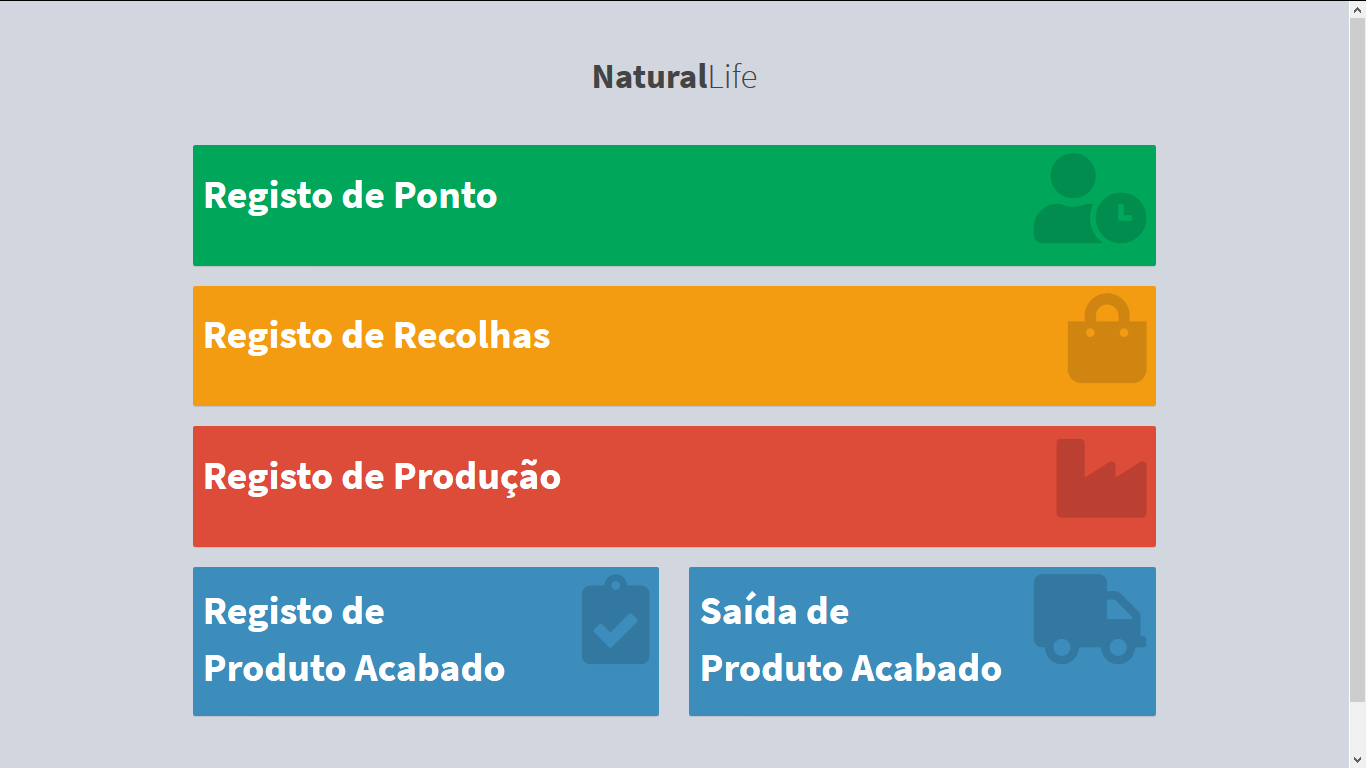
\includegraphics[width=0.90\textwidth,keepaspectratio]{figuras/AppPhp/0-menu_1_fase.png}
		\caption{Menú da Aplicação Fábrica na primeira fase}
		\label{fig:posinstall_fabrica_menu} 
	\end{center}
\end{figure}
\subsection{Primeiro dia de utilização}
O primeiro dia utilização foi a segunda-feira da semana oito, dia 3 de junho de 2019. Não foi detetado nenhum erro durante todo o dia, tendo sido apenas apontados detalhes de \textit{user experience}, por exemplo os colaboradores esperavam poder usar a virgula para separar as casas decimais no lugar do ponto. Apesar de não ser um requisito do sistema usar a virgula como separador das casas decimais essas modificações foram implementadas pois o trabalho necessário para as fazer era mínimo se comparado com a melhoria da \textit{user experience} dos colaboradores.

\subsection{Segunda fase de implementação}
Durante a segunda fase de implementação, as funcionalidades passaram a ser disponibilizadas após concluir o processo de teste. Este processo não era tão rigoroso como o da primeira fase, mas também não se fazia necessário porque deixou de existir a possibilidade da fábrica ser obrigada a parar por algum erro nas funcionalidades básicas da aplicação. No entanto as funcionalidades só passavam a estar disponíveis na versão em produção após o aval do supervisor. Foi nesta fase que alem de se desenvolver toda a aplicação Painel, foram implementadas as funcionalidades segunda via de código de barras e Completar recolha.

\subsection{Resultado do desenvolvimento}
De forma a se poder comparar diferenças entre o novo sistema e o atual fez-se a seguinte comparação.
Na figura \ref{fig:comparacao_menu} são apresentadas as diferenças entre o menu da aplicação anterior e o menu do novo sistema.
\begin{figure}[H]
	\centering
	
	\begin{subfigure}[t]{0.35\linewidth}
		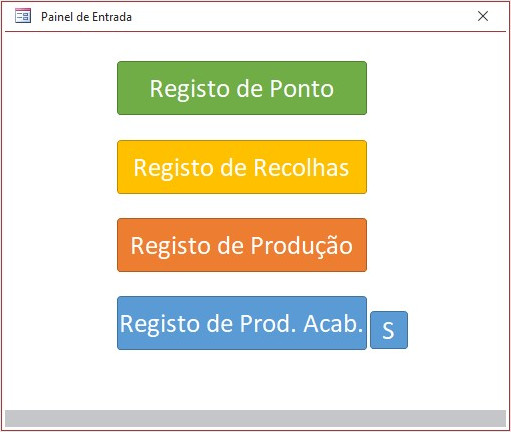
\includegraphics[width=\linewidth]{figuras/AppAccess/0-MenuInicial.jpg}
		\label{fig:comparacao_menu_1}
		\caption{Menu na aplicação anterior}
	\end{subfigure}
	\begin{subfigure}[t]{0.55\linewidth}
		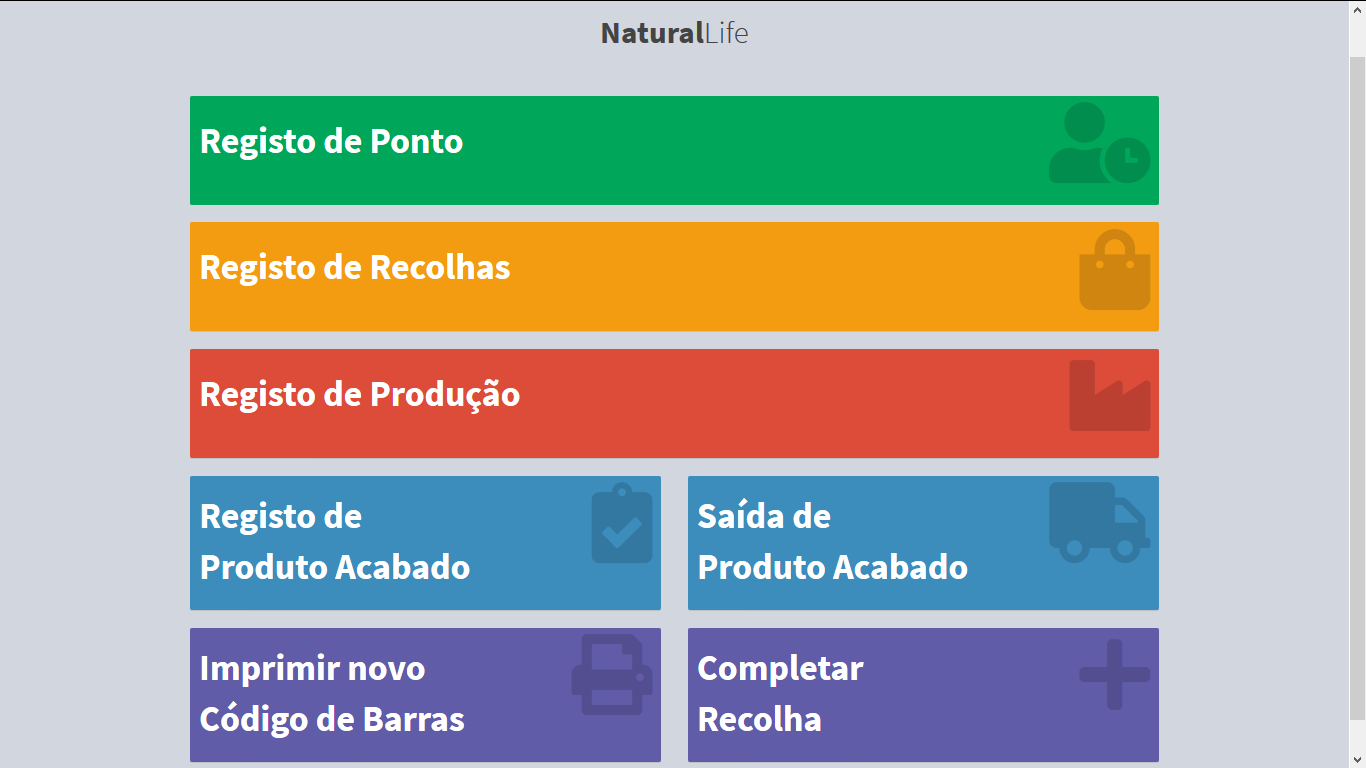
\includegraphics[width=\linewidth]{figuras/AppPhp/0-menu_2_fase.png}
		\label{fig:comparacao_menu_2}
		\caption{Menu na nova aplicação}
	\end{subfigure}
	
	\caption{Modelo do menu}
	\label{fig:comparacao_menu}
\end{figure}
\newpage
Na figura \ref{fig:comparacao_ponto} são apresentadas as diferenças entre a \textit{view} de registo de ponto da aplicação anterior e o do novo sistema.
\begin{figure}[H]
	\centering
	
	\begin{subfigure}[t]{0.3\linewidth}
		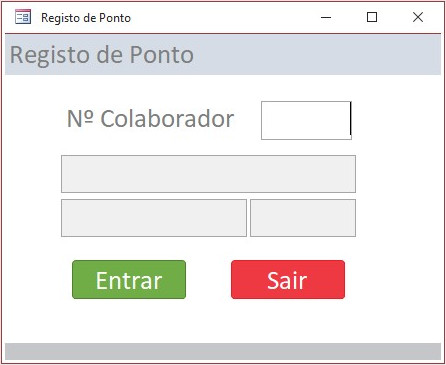
\includegraphics[width=\linewidth]{figuras/AppAccess/1-Ponto.jpg}
		\label{fig:comparacao_ponto_1}
		\caption{\textit{View} de registo de ponto na aplicação anterior}
	\end{subfigure}
	\begin{subfigure}[t]{0.60\linewidth}
		\includegraphics[width=\linewidth]{figuras/AppPhp/1_ponto.png}
		\label{fig:comparacao_ponto_2}
		\caption{\textit{View} de registo de ponto na nova aplicação}
	\end{subfigure}
	
	\caption{Registo de ponto}
	\label{fig:comparacao_ponto}
\end{figure}

Na figura \ref{fig:comparacao_recolha} são apresentadas as diferenças entre a \textit{view} de registo de recolha da aplicação anterior e o do novo sistema.
\begin{figure}[H]
	\centering
	
	\begin{subfigure}[t]{0.35\linewidth}
		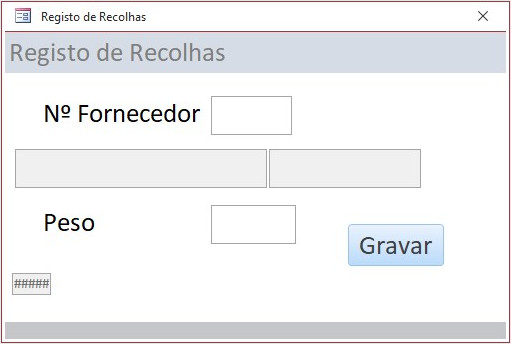
\includegraphics[width=\linewidth]{figuras/AppAccess/2-Recolha.jpg}
		\label{fig:comparacao_recolha_1}
		\caption{\textit{View} de registo de recolha na aplicação anterior}
	\end{subfigure}
	\begin{subfigure}[t]{0.55\linewidth}
		\includegraphics[width=\linewidth]{figuras/AppPhp/2_recolha.png}
		\label{fig:comparacao_recolha_2}
		\caption{\textit{View} de registo de recolha na nova aplicação}
	\end{subfigure}
	
	\caption{Registo de recolha}
	\label{fig:comparacao_recolha}
\end{figure}

Ainda relativamente ao registo de recolha, na figura \ref{fig:comparacao_recolhacb} são apresentadas as diferenças entre o código de barras gerado pela aplicação anterior e pelo novo sistema.
\begin{figure}[H]
	\centering
	
	\begin{subfigure}[t]{0.43\linewidth}
		
\includegraphics[width=\linewidth]{figuras/AppAccess/2-CodBarras.jpg}
		\label{fig:comparacao_recolhacb_1}
		\caption{código de barras gerado pela aplicação anterior}
	\end{subfigure}
	\begin{subfigure}[t]{0.48\linewidth}
		
\includegraphics[width=\linewidth]{figuras/AppPhp/2-CodBarras.png}
		\label{fig:comparacao_recolhacb_2}
		\caption{código de barras gerado pela nova aplicação}
	\end{subfigure}
	
	\caption{Códigos de barras da recolha}
	\label{fig:comparacao_recolhacb}
\end{figure}

Na figura \ref{fig:comparacao_producao} são apresentadas as diferenças entre a \textit{view} de registo de produção da aplicação anterior e o do novo sistema.
\begin{figure}[H]
	\centering
	
	\begin{subfigure}[t]{0.45\linewidth}
		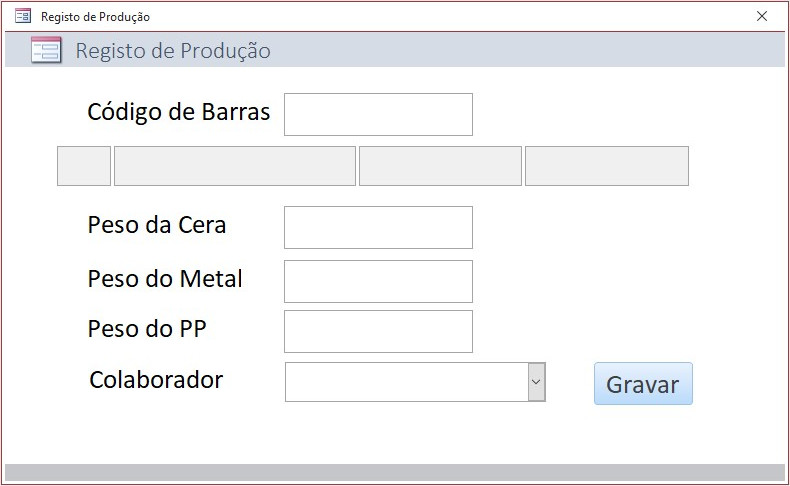
\includegraphics[width=\linewidth]{figuras/AppAccess/3-Producao.jpg}
		\label{fig:comparacao_producao_1}
		\caption{\textit{View} de registo de produção na aplicação anterior}
	\end{subfigure}
	\begin{subfigure}[t]{0.45\linewidth}
		\includegraphics[width=\linewidth]{figuras/AppPhp/3_producao.png}
		\label{fig:comparacao_producao_2}
		\caption{\textit{View} de registo de produção na nova aplicação}
	\end{subfigure}
	
	\caption{Registo de produção}
	\label{fig:comparacao_producao}
\end{figure}

Na figura \ref{fig:comparacao_prodacabado} são apresentadas as diferenças entre a \textit{view} de registo de produto acabado da aplicação anterior e o do novo sistema.
\begin{figure}[H]
	\centering
	
	\begin{subfigure}[t]{0.35\linewidth}
		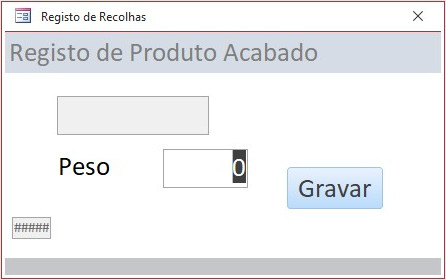
\includegraphics[width=\linewidth]{figuras/AppAccess/4-ProdutoAcabado.jpg}
		\label{fig:comparacao_prodacabado_1}
		\caption{\textit{View} de registo de produto acabado na aplicação anterior}
	\end{subfigure}
	\begin{subfigure}[t]{0.55\linewidth}
		\includegraphics[width=\linewidth]{figuras/AppPhp/4_produto_acabado.png}
		\label{fig:comparacao_prodacabado_2}
		\caption{\textit{View} de registo de produto acabado na nova aplicação}
	\end{subfigure}
	
	\caption{Registo de produto acabado}
	\label{fig:comparacao_prodacabado}
\end{figure}

Ainda relativamente ao registo de produto acabado, na figura \ref{fig:comparacao_prodacabadocb} são apresentadas as diferenças entre o código de barras gerado pela aplicação anterior e pelo novo sistema.
\begin{figure}[H]
	\centering
	
	\begin{subfigure}[t]{0.45\linewidth}
		
\includegraphics[width=\linewidth]{figuras/AppAccess/5-CodBarras.jpg}
		\label{fig:comparacao_prodacabadocb_1}
		\caption{código de barras gerado pela aplicação anterior}
	\end{subfigure}
	\begin{subfigure}[t]{0.45\linewidth}
		
\includegraphics[width=\linewidth]{figuras/AppPhp/5-CodBarras.png}
		\label{fig:comparacao_prodacabadocb_2}
		\caption{código de barras gerado pela nova aplicação}
	\end{subfigure}
	
	\caption{Códigos de barras do produto acabado}
	\label{fig:comparacao_prodacabadocb}
\end{figure}

Na figura \ref{fig:comparacao_prodacabado_saida} são apresentadas as diferenças entre a \textit{view} de registo de saída de produto acabado da aplicação anterior e o do novo sistema.
\begin{figure}[H]
	\centering
	
	\begin{subfigure}[t]{0.40\linewidth}
		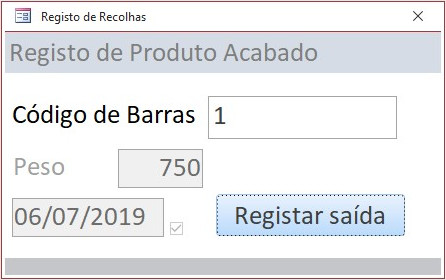
\includegraphics[width=\linewidth]{figuras/AppAccess/5-SaidaProdutoAcabado.jpg}
		\label{fig:comparacao_prodacabado_saida_1}
		\caption{\textit{View} de registo de produto acabado na aplicação anterior}
	\end{subfigure}
	\begin{subfigure}[t]{0.50\linewidth}
		\includegraphics[width=\linewidth]{figuras/AppPhp/5_saida_produto_acabado_2_fase.png}
		\label{fig:comparacao_prodacabado_saida_2}
		\caption{\textit{View} de registo saída de produto acabado na nova aplicação}
	\end{subfigure}
	
	\caption{Registo de saída de produto acabado}
	\label{fig:comparacao_prodacabado_saida}
\end{figure}

Na figura \ref{fig:comparacao_novasfunc} são apresentadas as funcionalidades segunda via e completar recolha que não existiam no sistema anterior.
\begin{figure}[H]
	\centering
	
	\begin{subfigure}[t]{0.45\linewidth}
		\includegraphics[width=\linewidth]{figuras/AppPhp/6_2_via.png}
		\label{fig:comparacao_novasfunc_1}
		\caption{\textit{View} do pedido de segunda via de código de barras}
	\end{subfigure}
	\begin{subfigure}[t]{0.45\linewidth}
		\includegraphics[width=\linewidth]{figuras/AppPhp/7_completar_recolha.png}
		\label{fig:comparacao_novasfunc_2}
		\caption{\textit{View} do incremento de uma recolha}
	\end{subfigure}
	
	\caption{Funcionalidades inexistentes no sistema anterior}
	\label{fig:comparacao_novasfunc}
\end{figure}

Outro elemento que não existia na aplicação anterior era o Painel. Nas figura \ref{fig:comparacao_paine_l} e \ref{fig:comparacao_painel} são apresentadas as funcionalidades listagem, inserção e edição.
\begin{figure}[H]
	\centering
	
	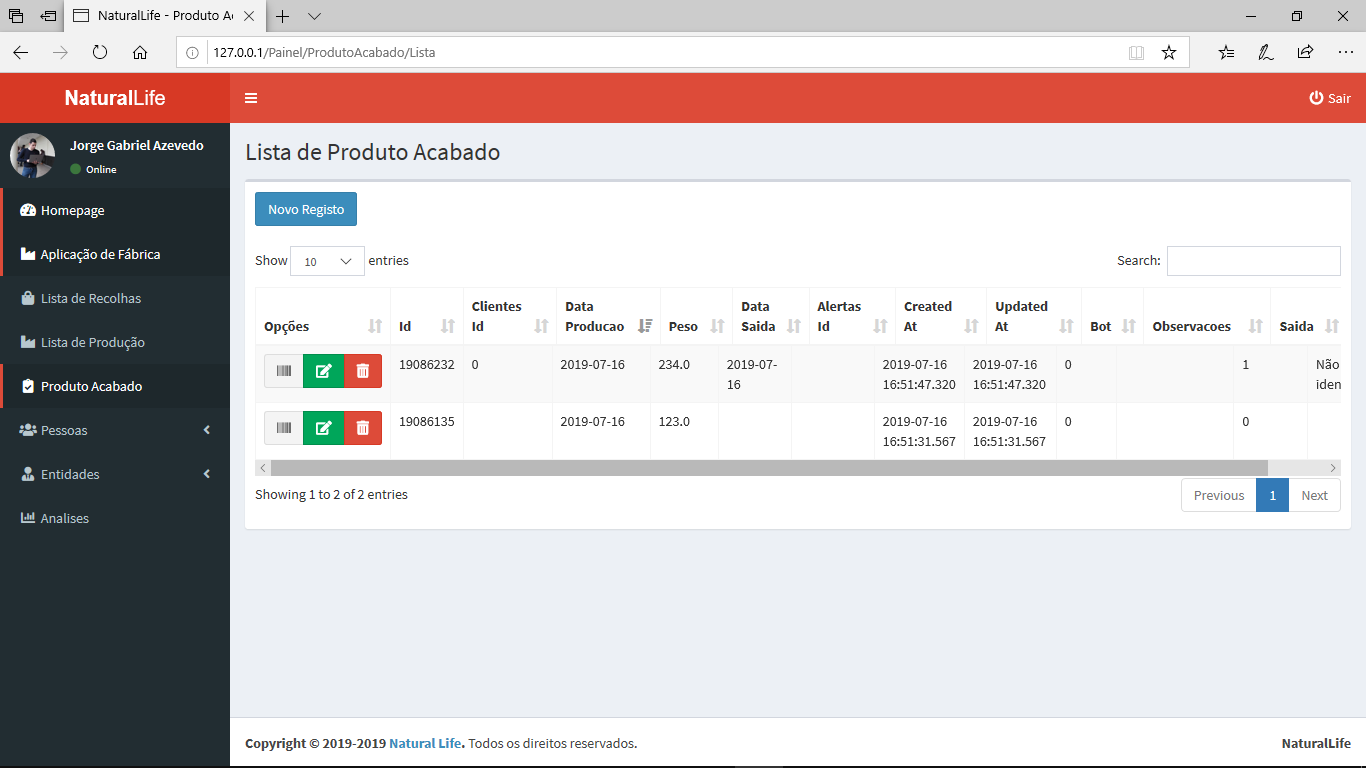
\includegraphics[width=0.7\linewidth]{figuras/AppPhp/8-lista.png}
	\label{fig:comparacao_painel_l}
	\caption{Exemplo de \textit{View} listagem}

\end{figure}
\begin{figure}[H]
	\centering
	\begin{subfigure}[t]{0.45\linewidth}
		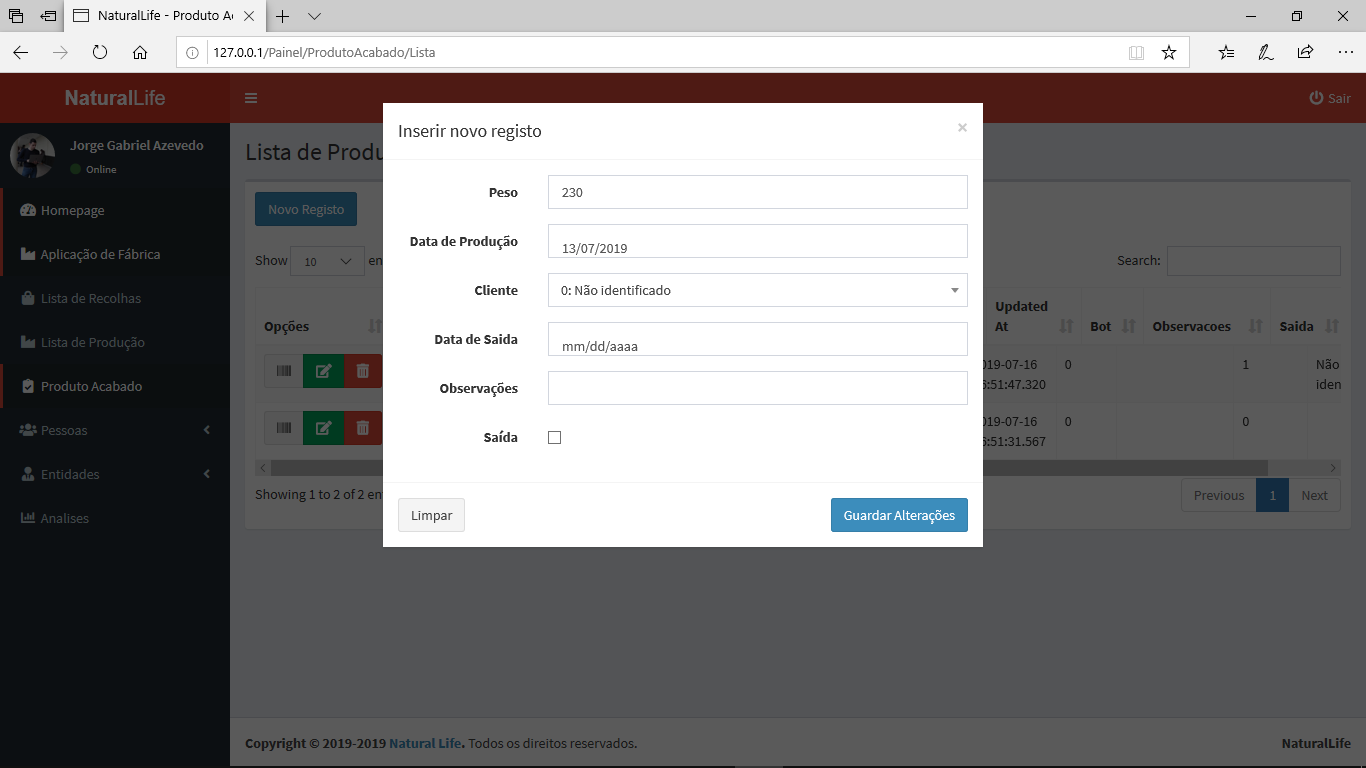
\includegraphics[width=\linewidth]{figuras/AppPhp/9-novo.png}
		\label{fig:comparacao_painel_1}
		\caption{Exemplo de \textit{View} inserção}
	\end{subfigure}
	\begin{subfigure}[t]{0.45\linewidth}
		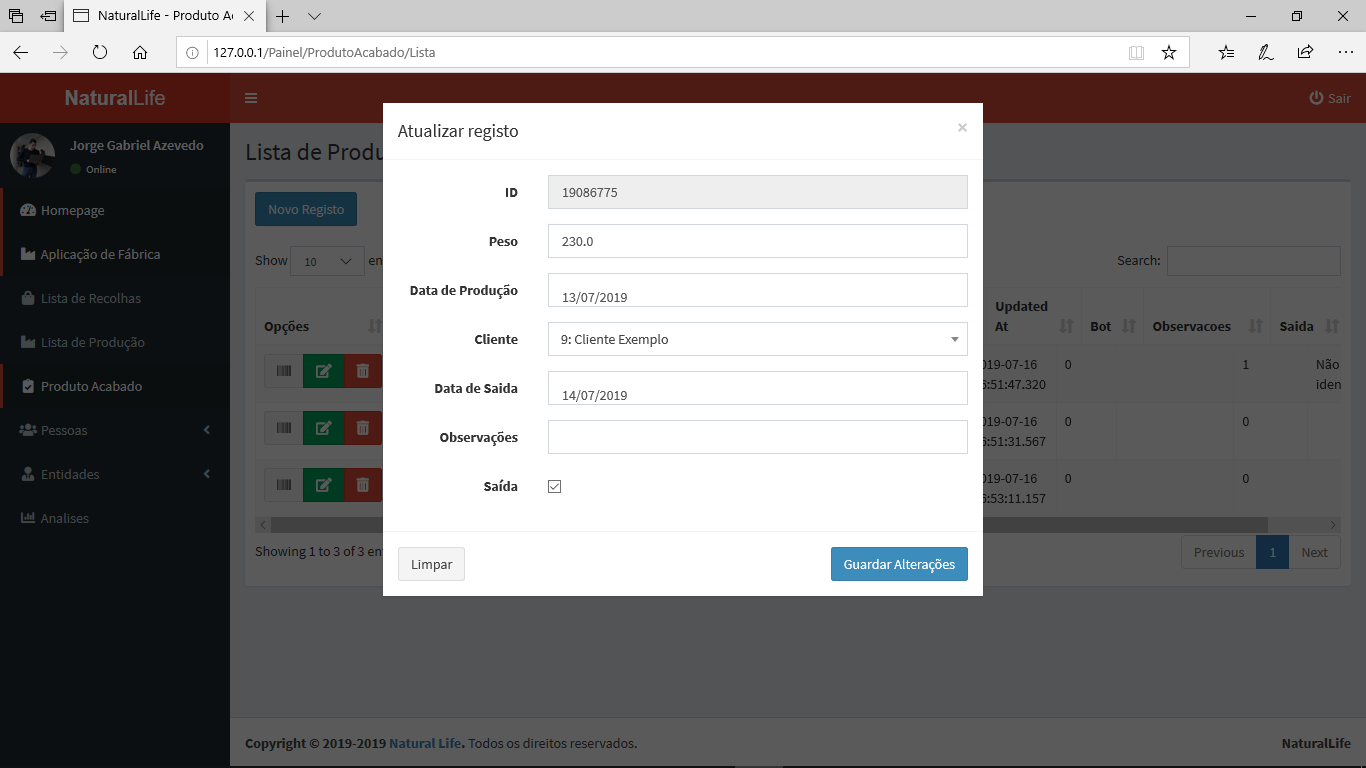
\includegraphics[width=\linewidth]{figuras/AppPhp/10-editar.png}
		\label{fig:comparacao_painel_2}
		\caption{Exemplo de \textit{View} edição}
	\end{subfigure}
	
	\caption{\textit{View} da Aplicação Painel}
	\label{fig:comparacao_painel}
\end{figure}

\section{Validação do trabalho}
Logo desde a primeira fase de implementação notou-se uma grande satisfação por parte da administração da Natural Life. Este sentimento foi-se mantendo até ao final do estágio, momento no qual a empresa confirmou que a aplicação iria continuar a ser utilizada na empresa. Consultado o supervisor sobre a poupança de tempo semanal com a implementação deste sistema este referiu uma redução de 20\% a 30\% do tempo de trabalho semanal a efetura confirmação e retificação de registos.\\
Da perspetiva dos colaboradores, o \textit{feedback} também foi muito positivo. O maior receio da administração seria que estes não se adaptassem ao novo sistema e houvesse a necessidade de retornar ao anterior. Mas a verdade é que a reação foi bem melhor do que era espectado. A reação por parte dos colaboradores foi de enorme agrado, havendo inclusivamente lugar a sugestões de melhoria feitas à administração.
\newpage
\section{Execução do projeto} 
Como forma de avaliar o desenvolvimento do projeto, foi construído um gráfico da figura \ref{fig:burndown_chart}, denominado \textit{burndown char}, que demonstra a relação entre os objetivos a cumprir com o período do projeto.

\begin{figure}[H] 
	\begin{center}
		% Requires \usepackage{graphicx}
		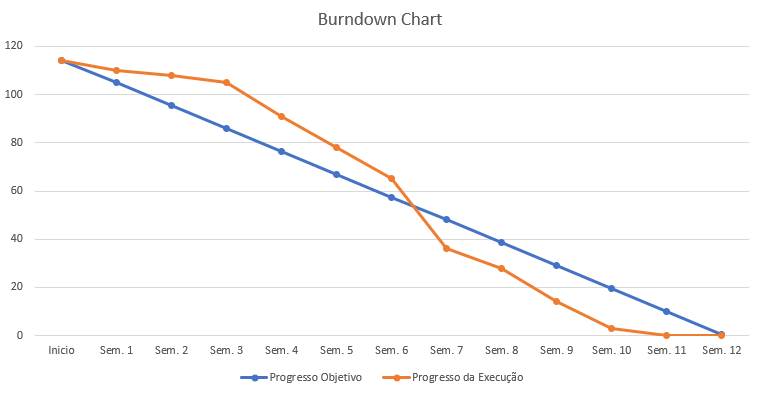
\includegraphics[width=0.90\textwidth,keepaspectratio]{figuras/burndown_chart.png}
		\caption{\textit{burndown char} da excussão do projeto}
		\label{fig:burndown_chart} 
	\end{center}
\end{figure}

\noindent
A linha de cor azul refere-se ao que era espectável que acontecesse, um desenvolvimento constante no qual o projeto é entregue no último dia do período, com todos os objetivos concluídos. A laranja é possível observar a evolução real do trabalho. Desta linha é relevante analisar que durante as primeiras três semana a evolução do projeto ficou à quem do esperado, mas após a terceira semana a linha de execução superou a previsão culminando com a conclusão do projeto uma semana antes do previsto. A razão para a diferença entre as duas linhas prende-se com o facto de que nas primeiras três semanas terem sido semanas de estudo e adaptação. Concluído esse processo já tinham sido construídos as ferramentas necessárias para a execução do projeto.

\section{\textit{Software}s e serviços usados}
O projeto possuía um conjunto tão alagado de requisitos que para proceder à sua elaboração foi necessário utilizar um grande conjunto de \textit{software}s e serviços. Desta lista fazem partes, sistemas operativos, editores de código, servidores, DBMSs, linguagens de programação e restantes utilitários.

\begin{multicols}{3}
	\begin{itemize}
		\item Microsoft Windows 10
		\item Ubuntu 18.04
		
		\item Apache
		\item Microsoft SQL Server
		
		\item Microsoft Database Management Studio
		\item Microsoft Visual Studio
		
		\item PHP
		\item Laravel
		\item AdminLTE
		\item JavaScript
		\item JQuery
		
		\item Microsoft Excel
		\item Microsoft Access
		\item Microsoft Excel
		\item Microsoft Word
		
		\item Visual Paradigm
		\item Draw.io
		
		\item Trello
		\item GitHub
		\item Git
		\item GitKraken
		
		\item \LaTeX
		\item Overleaf.com
		\item Microsoft Excel
	\end{itemize}
\end{multicols}

Segundo dados da plataforma GitHub foram feitos 377 \textit{commits}, contabilizando aproximadamente 115 500 linhas de código escritas.